\input{LectureSlides/includes/metropolis_preamble}

% Title page info
\title[Expected Utility]{Chapter 5: Expected Utility Theory}
\author[ECON 5001]{ECON 5001\\Prof. Paul J. Healy\\Based on: \textit{Game Theory} by Giacomo Bonanno} \color{metrop}
\institute[OSU]{}
\date[]{\vfill {\tiny Updated \today\ at\ \DTMcurrenttime}}

% ---------------------------------------------------------------------
% NOTATION IN THIS DECK (differs from Bonanno on purpose):
%   u(o)  small u:   the "utility index" over OUTCOMES
%   U(L)  capital U: the "expected utility" over LOTTERIES
% Bonanno writes U(o) for the first and E[U(L)] for the second.
% We say "linear rescaling" for v = a*u + b with a>0. Bonanno's term
% ("positive affine transformation") appears once, in a footnote.
% The vNM axioms (Section 5.3) are mentioned but not taught.
%
% Two things here are NOT in Bonanno and are flagged on the slides:
%   (1) risk attitudes are only defined for numeric outcomes
%   (2) risk averse / neutral / loving <=> u concave / linear / convex
%
% Curves in the risk-attitude pictures are schematic (drawn extra curvy
% so the gap between U(L) and u(15) is visible). Through ($10, 1.64) and
% ($20, 4.33) in all three panels; chord midpoint is ($15, 2.985).
% ---------------------------------------------------------------------

% Axes + chord + dotted guides shared by the three risk-attitude pictures.
% #1 = curve as a pgf expression in \x (dollars), #2 = plot domain,
% #3 = height of the curve at $15
\newcommand{\riskpanel}[3]{%
  \draw[->] (7,0) -- (25.5,0) node[below] {\scriptsize \$};
  \draw[->] (7,0) -- (7,6.2) node[left] {\scriptsize $u$};
  \draw[blue, very thick, smooth, samples=80, domain=#2] plot (\x,{#1});
  \draw[thick] (10,1.64) -- (20,4.33);
  \foreach \d in {10,15,20}{
    \draw (\d,0.1) -- (\d,-0.1) node[below] {\scriptsize \d};
  }
  \draw[dotted, thick] (10,0) -- (10,1.64);
  \draw[dotted, thick] (20,0) -- (20,4.33);
  \draw[dotted, thick] (15,0) -- (15,#3);
  \draw[dotted, thick] (15,0) -- (15,2.985);
  \fill (10,1.64) circle (1.6pt);
  \fill (20,4.33) circle (1.6pt);
  \fill[red] (15,2.985) circle (2pt);
  \fill[blue] (15,#3) circle (2pt);
}

\begin{document}

\frame{\maketitle}

\begin{frame}{Beyond Risk Neutrality}
Chapter 4: chance moves give us \textbf{lotteries} over outcomes\\
Our shortcut was to assume:
\begin{itemize}
    \item All outcomes are money
    \item Players are \textbf{risk neutral} (rank lotteries by expected value)
\end{itemize}
\bsk
That leaves out a lot:
\begin{itemize}
    \item People buy insurance. (And lottery tickets!)
    \item Many outcomes aren't money at all
    \begin{itemize}
        \item Win/lose/draw, getting the job, where to eat dinner...
    \end{itemize}
\end{itemize}
\vfill
Our goal:
\begin{enumerate}
    \item Rank lotteries over \textbf{any} kind of outcome
    \item Describe different attitudes toward risk
\end{enumerate}
\vspace{-0.4in}
\end{frame}

% ==============================================================
% MOBLAB --- PLAY FIRST
% ==============================================================

% ---- MobLab run: Risk Preferences: Bomb Risk Game --------------------
% Topic: Decision Making. 100 boxes, one hides a bomb. Each student picks
% how many boxes to open. Earnings = number opened, or 0 if the bomb is
% among them. Results screen gives min / max / median and a histogram.
% Expected earnings from opening k boxes: k(100-k)/100, maximized at 50.
% Play BEFORE risk attitudes are defined. Comes back in "Back to the
% Bomb Game".
% ---------------------------------------------------------------------
\begin{frame}{MobLab: ``Bomb Risk Game''}
\begin{itemize}
    \item MobLab time!
    \item There are 100 boxes. One of them hides a \textbf{bomb}
    \begin{itemize}
        \item Every box is equally likely to have it
    \end{itemize}
    \item You choose how many boxes to open (anything from 0 to 100)
    \item Then we find out where the bomb was:
    \begin{itemize}
        \item \textbf{Not} in your boxes: you earn 1 point per box you opened
        \item \textbf{In} your boxes: you earn 0
    \end{itemize}
\end{itemize}
\bsk
\vfill
\centering
Feel free to talk! And play it the way you'd actually play it.
\vspace{-0.3in}
\end{frame}

% \begin{frame}{How Many Boxes?}
% \vspace{0.5in}
% \centering
% \begin{tabular}{lc}
% Fewest boxes opened: & \underline{\hspace{1in}} \\[0.3in]
% Median \# of boxes opened: & \underline{\hspace{1in}} \\[0.3in]
% Most boxes opened: & \underline{\hspace{1in}} \\[0.3in]
% \end{tabular}
% \end{frame}

% ==============================================================
% LOTTERIES AND EXPECTED VALUE
% ==============================================================

\begin{frame}[standout]
Lotteries
\end{frame}

\begin{frame}{Lotteries}
A \textbf{lottery} $L$ is a list of outcomes and their probabilities:
$$L=\begin{pmatrix} o_1 & o_2 & \cdots & o_n \\ p_1 & p_2 & \cdots & p_n\end{pmatrix}$$
\bsk
The outcomes can be \textbf{anything}:
\bsk
\begin{itemize}
    \item Money: \hspace{0.45in}
      $L_1=\begin{pmatrix} \$10 & \$20 \\[2pt] \tfrac12 & \tfrac12\end{pmatrix}$
      \vspace{0.2in}
    \item Not money: \hspace{0.2in}
      $L_2=\begin{pmatrix} \text{Buckeyes beat Michigan} & \text{Buckeyes lose to Michigan} \\[2pt] \tfrac35 & \tfrac25\end{pmatrix}$
\end{itemize}
\vfill
A sure thing is a lottery too. Just write $o$ for ``outcome $o$ with probability 1''
\vspace{-0.3in}
\end{frame}

\begin{frame}{Expected Value: Numbers Only}
Recall the \textbf{expected value} of a money lottery:
$$E[L] = p_1x_1 + p_2x_2 + \cdots + p_nx_n$$
\bsk
$L_1=\begin{pmatrix} \$10 & \$20 \\[2pt] \tfrac12 & \tfrac12\end{pmatrix}$
\hspace{0.3in} $E[L_1]=$ \underline{\hspace{1.5in}}
\bsk
$L_2=\begin{pmatrix} \text{Beat Michigan} & \text{Lose to Michigan} \\[2pt] \tfrac35 & \tfrac25\end{pmatrix}$
\hspace{0.3in} $E[L_2]=$ \onslide<2->{???}
\vfill
\onslide<3->{\textbf{Lesson:} We can calculate an expected value when outcomes are \textbf{numbers} (like money).\\
When outcomes are \textbf{not} numbers, expected value doesn't exist!
\bsk
So how do we rank lotteries like $L_2$?}
\vspace{-0.3in}
\end{frame}

% ==============================================================
% 5.2 EXPECTED UTILITY
% ==============================================================

\begin{frame}[standout]
Expected Utility
\end{frame}

\begin{frame}{Two Kinds of Utility}
\textbf{Step 1:} Give every \textit{outcome} a number
\begin{itemize}
    \item $u(o)$ is the \textbf{utility index} of outcome $o$ \hfill (small $u$: outcomes)
\end{itemize}
\bsk
\textbf{Step 2:} Use those to give every \textit{lottery} a number
\begin{itemize}
    \item $U(L)$ is the \textbf{expected utility} of lottery $L$ \hfill (capital $U$: lotteries)
\end{itemize}
\bsk
Expected utility: average the utility index, weighting by the probabilities.
\bsk
$$\underbrace{U(L)\vphantom{p_1}}_{\text{expected utility of the lottery}}\ =\ \underbrace{p_1u(o_1)+p_2u(o_2)+\cdots+p_nu(o_n)}_{\text{probability-weighted average of the utility index}}$$
\vfill
{\footnotesize Bonanno writes $U(o)$ for our $u(o)$, and $E[U(L)]$ for our $U(L)$.}
\vspace{-0.2in}
\end{frame}

\begin{frame}{Example}
Alex's utility index over dinner outcomes:
\bsk
\centering
\begin{tabular}{r|c|c|c|}
\cline{2-4}
Outcome $o$ & Cazuela's & Yoshi Sushi & Dining hall \\
\cline{2-4}
Utility index $u(o)$ & $10$ & $6$ & $0$ \\
\cline{2-4}
\end{tabular}
\bsk
\raggedright
Two lotteries:
$$L_A=\begin{pmatrix} \text{Yoshi Sushi} \\[2pt] 1\end{pmatrix}
\qquad\qquad
L_B=\begin{pmatrix} \text{Cazuela's} & \text{Dining hall} \\[2pt] \tfrac12 & \tfrac12\end{pmatrix}$$
\bsk
$U(L_A)=$ \hspace{2.2in} $U(L_B)=$
\vfill
Alex prefers: \underline{\hspace{1in}}
\bsk
Note: no expected \textit{value} here. But expected \textit{utility} works fine.
\vspace{-0.3in}
\end{frame}

\begin{frame}{Why Expected Utility?}
Do people really rank lotteries by expected utility?
\bsk
\begin{block}{Theorem (von Neumann \& Morgenstern, 1944)}
If your ranking of lotteries satisfies a few ``rationality'' axioms, then there is a utility index $u(o)$ such that
$$L\succ L' \iff U(L)>U(L') \qquad\text{and}\qquad L\sim L' \iff U(L)=U(L')$$
\end{block}
\bsk
In words: you act \textit{as if} you're maximizing expected utility
\bsk
The axioms are in Bonanno \S5.3. We're going to skip them.
\begin{itemize}
    \item Interested? Read through them for fun!
\end{itemize}
\vfill
From here on: we \textbf{assume} players maximize expected utility
\vspace{-0.4in}
\end{frame}

% ---- Historical figure slide ------------------------------------------
% Portraits are in the ECON 8877 project (graphics/history). Copy them to
% LectureSlides/graphics/history/ under the two names below, downsampled
% to ~600px tall. Until then the slide compiles without them.
\begin{frame}{von Neumann \& Morgenstern}
\IfFileExists{LectureSlides/graphics/history/vonNeumannMug.png}{%
\centering
\begin{tabular}{c@{\hspace{0.6in}}c}
\includegraphics[height=1.05in]{LectureSlides/graphics/history/vonNeumannMug.png} &
\includegraphics[height=1.05in]{LectureSlides/graphics/history/MorgensternMug.png} \\[0.04in]
{\small John von Neumann (1903--1957)} & {\small Oskar Morgenstern (1902--1977)}
\end{tabular}
\bsk
\raggedright
}{}
\begin{itemize}
    \item \textbf{von Neumann}: Budapest math prodigy. Princeton IAS (with Einstein)
    \begin{itemize}
        \item Manhattan Project, modern computer design, minimax theorem
    \end{itemize}
    \item \textbf{Morgenstern}: Vienna economist. Left Austria in 1938
    \item \textbf{1944}: \textit{Theory of Games and Economic Behavior}. Game theory is born
    \item Expected utility axioms: an appendix to the 1947 edition!
\end{itemize}
\vspace{-0.2in}
\end{frame}

% ==============================================================
% RESCALING AND NORMALIZING
% ==============================================================

\begin{frame}[standout]
Rescaling the Utility Index
\end{frame}

\begin{frame}{Can We Rescale Any Way We Want?}
\textbf{Chapter 2:} utility only \textit{ranked} outcomes. Any increasing rescaling was fine.
\bsk
Is that still true? Try squaring Alex's utility index: \ $v(o)=u(o)^2$
\bsk
\centering
\begin{tabular}{r|c|c|c|}
\cline{2-4}
Outcome $o$ & Cazuela's & Yoshi Sushi & Dining hall \\
\cline{2-4}
$u(o)$ & $10$ & $6$ & $0$ \\
\cline{2-4}
$v(o)=u(o)^2$ & $100$ & $36$ & $0$ \\
\cline{2-4}
\end{tabular}
\bsk
\raggedright
Using $v$: \hspace{0.3in} $V(L_A)=$ \hspace{1.6in} $V(L_B)=$
\bsk
\onslide<2->{Same ranking of \textit{outcomes}. Different ranking of \textit{lotteries}!!}
\vfill
\onslide<2->{\textbf{Lesson:} The utility index can \textbf{not} be rescaled arbitrarily}
\vspace{-0.3in}
\end{frame}

\begin{frame}{Linear Rescaling}
Which rescalings \textit{are} allowed? Only \textbf{linear} ones:
$$v(o)=a\cdot u(o)+b \qquad (\text{with } a>0)$$
\begin{itemize}
    \item You can \textbf{multiply} by a positive number $a$
    \item You can \textbf{add} (or subtract) a constant $b$
\end{itemize}
\bsk
Try $v(o)=2u(o)+3$ on Alex's index $(10,6,0)$:
\bsk
$v=($\hspace{1in}$)$ \hspace{0.4in} $V(L_A)=$ \hspace{1in} $V(L_B)=$
\bsk
\textbf{Theorem:} $u$ and $v$ rank all lotteries the same way $\iff$ $v$ is a linear rescaling of $u$
\bsk
Like temperature: \ ${}^\circ\text{F} = 1.8\times{}^\circ\text{C}+32$. \ Different numbers, same information.
\vfill
{\footnotesize Bonanno calls a linear rescaling a ``positive affine transformation.''}
\vspace{-0.2in}
\end{frame}

\begin{frame}{Normalizing}
Since linear rescaling is allowed, we can always pick a convenient scale:
\bsk
\centering
\large
$u(\text{best outcome})=1$ \qquad\qquad $u(\text{worst outcome})=0$
\normalsize
\bsk
\raggedright
This is called the \textbf{normalized} utility index. How to get it:
\begin{enumerate}
    \item Subtract $u(\text{worst})$ from every number \hfill (now the worst is 0)
    \item Divide every number by the new $u(\text{best})$ \hfill (now the best is 1)
\end{enumerate}
\bsk
\centering
\renewcommand{\arraystretch}{1.5}
\begin{tabular}{r|c|c|c|c|}
\cline{2-5}
Outcome & $o_1$ & $o_2$ & $o_3$ & $o_4$ \\
\cline{2-5}
$u(o)$ & $8$ & $2$ & $-2$ & $0$ \\
\cline{2-5}
After step 1 & \hspace{0.5in} & \hspace{0.5in} & \hspace{0.5in} & \hspace{0.5in} \\
\cline{2-5}
After step 2 & & & & \\
\cline{2-5}
\end{tabular}
\end{frame}

% \begin{frame}{What the Normalized Numbers Mean}
% With a normalized index, the numbers have a nice interpretation.
% \bsk
% Take a lottery over just the best and worst outcomes:
% $$L=\begin{pmatrix} o_{\text{best}} & o_{\text{worst}} \\[2pt] p & 1-p\end{pmatrix}
% \qquad\Rightarrow\qquad U(L)=p\,(1)+(1-p)\,(0)=p$$
% \bsk
% So $u(o)=0.4$ means:
% \begin{itemize}
%     \item Getting $o$ for sure is exactly as good as a \textbf{40\% chance at the best outcome}\\
%       (and a 60\% chance of the worst)
% \end{itemize}
% \bsk
% This also tells us how to \textit{find} someone's utility index. Just ask them:
% \begin{center}
% ``What chance $p$ of the best outcome is just as good as $o$ for sure?''
% \end{center}
% Their answer is $u(o)$.
% \vspace{-0.2in}
% \end{frame}

% ==============================================================
% 5.1 ATTITUDES TO RISK
% ==============================================================

\begin{frame}[standout]
Attitudes Toward Risk
\end{frame}

\begin{frame}{Risk Averse, Risk Neutral, Risk Loving}
Back to \textbf{money} lotteries, where $E[L]$ exists. Offer someone a choice:
\bsk
\centering
the lottery $L$ \qquad vs. \qquad getting $\$E[L]$ for sure
\bsk
\raggedright
\begin{block}{Definition}
\begin{itemize}
    \item \textbf{Risk averse}: prefers $\$E[L]$ for sure
    \item \textbf{Risk neutral}: indifferent between them
    \item \textbf{Risk loving}: prefers the lottery $L$
\end{itemize}
\end{block}
\bsk
\textbf{Ex:} \ $L_1=\begin{pmatrix} \$10 & \$20 \\[2pt] \tfrac12 & \tfrac12\end{pmatrix}$ \ vs. \ \$15 for sure. \ Which would you take?
\vfill
\textbf{Important:} This only makes sense when outcomes are \textbf{numbers} (like money).\\
No $E[L]$ means no ``risk averse'' or ``risk loving.'' {\footnotesize (Bonanno doesn't say this.)}
\vspace{-0.3in}
\end{frame}

\begin{frame}{Risk Attitudes and the Shape of $u(o)$}
With expected utility, the definition becomes a comparison of two numbers:
\bsk
$$\underbrace{U(L)}_{\text{expected utility of the lottery}}
\qquad\text{vs.}\qquad
\underbrace{u\big(E[L]\big)}_{\text{utility of the expected value}}$$
\bsk
\centering
\renewcommand{\arraystretch}{1.7}
\begin{tabular}{lcccc}
\textbf{Risk averse} & $\iff$ & $U(L)<u\big(E[L]\big)$ & $\iff$ & $u(o)$ is \textbf{concave} \\
\textbf{Risk neutral} & $\iff$ & $U(L)=u\big(E[L]\big)$ & $\iff$ & $u(o)$ is \textbf{linear} \\
\textbf{Risk loving} & $\iff$ & $U(L)>u\big(E[L]\big)$ & $\iff$ & $u(o)$ is \textbf{convex} \\
\end{tabular}
\vfill
\raggedright
{\footnotesize This isn't in Bonanno, but it's how economists usually think about risk attitudes.}
\vspace{-0.2in}
\end{frame}

\begin{frame}{Risk Averse $\iff$ Concave}
\centering
\begin{tikzpicture}[x=0.5cm, y=0.82cm, >=stealth]
  \draw[->] (7,0) -- (25.5,0) node[below] {\small money (\$)};
  \draw[->] (7,0) -- (7,6.2) node[above] {\small utility index $u(o)$};
  \draw[blue, very thick, smooth, samples=80, domain=8.75:25] plot (\x,{1.5*ln(\x-8)+0.6});
  \foreach \d in {10,20}{ \draw (\d,0.1) -- (\d,-0.1) node[below] {\small \$\d}; }
  \draw[dotted, thick] (10,0) -- (10,1.64) -- (7,1.64) node[left] {\small $u(10)$};
  \draw[dotted, thick] (20,0) -- (20,4.33) -- (7,4.33) node[left] {\small $u(20)$};
  \fill (10,1.64) circle (2pt);
  \fill (20,4.33) circle (2pt);
  \onslide<2->{
    \draw[thick] (10,1.64) -- (20,4.33);
    \draw (15,0.1) -- (15,-0.1) node[below] {\small \$15};
    \draw[dotted, thick, red] (15,0) -- (15,2.985) -- (7,2.985)
      node[left] {\small $U(L_1)=\tfrac12u(10)+\tfrac12u(20)$};
    \fill[red] (15,2.985) circle (2.4pt);
  }
  \onslide<3->{
    \draw[dotted, thick, blue] (15,2.985) -- (15,3.52) -- (7,3.52) node[left] {\small $u(15)$};
    \fill[blue] (15,3.52) circle (2.4pt);
  }
\end{tikzpicture}
\bsk
\raggedright
\only<1>{$L_1$ pays \$10 or \$20 with equal chance. \ $E[L_1]=\$15$.}%
\only<2>{$U(L_1)$ is halfway up between $u(10)$ and $u(20)$: the midpoint of the straight line.}%
\only<3>{The curve is \textit{above} the line, so $u(15)>U(L_1)$. \ They'd rather have \$15 for sure.}
\vspace{-0.2in}
\end{frame}

\begin{frame}{All Three Cases}
\begin{columns}[T]
\begin{column}{0.32\textwidth}
\centering
\textbf{Concave}\\[4pt]
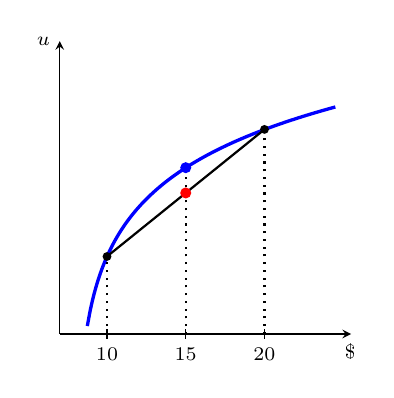
\begin{tikzpicture}[x=0.2cm, y=0.6cm, >=stealth]
  \riskpanel{1.5*ln(\x-8)+0.6}{8.75:24.5}{3.52}
\end{tikzpicture}\\[4pt]
$\color{red}U(L_1)\color{black}<\color{blue}u(15)$\\[4pt]
Risk averse
\end{column}
\begin{column}{0.32\textwidth}
\centering
\textbf{Linear}\\[4pt]
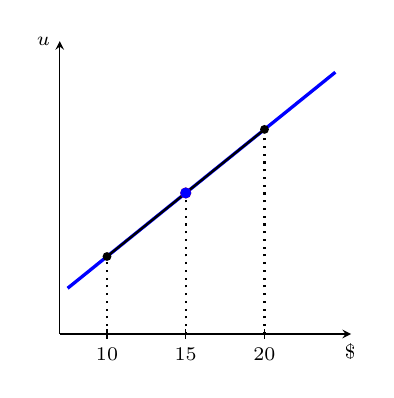
\begin{tikzpicture}[x=0.2cm, y=0.6cm, >=stealth]
  \riskpanel{1.64+0.269*(\x-10)}{7.5:24.5}{2.985}
\end{tikzpicture}\\[4pt]
$\color{red}U(L_1)\color{black}=\color{blue}u(15)$\\[4pt]
Risk neutral
\end{column}
\begin{column}{0.32\textwidth}
\centering
\textbf{Convex}\\[4pt]
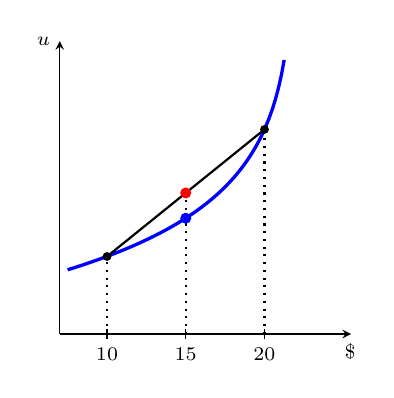
\begin{tikzpicture}[x=0.2cm, y=0.6cm, >=stealth]
  \riskpanel{5.37-1.5*ln(22-\x)}{7.5:21.25}{2.45}
\end{tikzpicture}\\[4pt]
$\color{red}U(L_1)\color{black}>\color{blue}u(15)$\\[4pt]
Risk loving
\end{column}
\end{columns}
\bsk
\centering
{\color{red}Red dot}: expected utility of the lottery. \ {\color{blue}Blue dot}: utility of \$15 for sure.
\end{frame}

\begin{frame}{Back to the Bomb Game}
Open $k$ boxes: you earn $k$ with probability $\tfrac{100-k}{100}$, otherwise 0
\bsk
Expected value: \ $E[L_k]=k\cdot\dfrac{100-k}{100}$
\bsk
\begin{itemize}
    \item Biggest when $k=$ \underline{\hspace{0.6in}} \vspace{0.15in}
    \item Opening \textbf{exactly} that many: risk \underline{\hspace{1in}} \vspace{0.15in}
    \item Opening \textbf{fewer}: risk \underline{\hspace{1in}} \vspace{0.15in}
    \item Opening \textbf{more}: risk \underline{\hspace{1in}} \vspace{0.15in}
\end{itemize}
Our class median: \underline{\hspace{1in}}
\vfill
\textbf{Lab result:} the typical person opens a bit fewer than 50\\
{\footnotesize Source: Crosetto \& Filippin (2013), \textit{Journal of Risk and Uncertainty}.}
\vspace{-0.2in}
\end{frame}

\begin{frame}{Risk Attitudes in the Real World}
Lots of real decisions boil down to ``lottery vs. sure thing'':
\bsk
\begin{itemize}
    \item \textbf{Insurance.} Pay a premium for sure, or risk a big loss?
    \item \textbf{Extended warranties.} Same thing, for your laptop
    \item \textbf{Salary vs.\ commission.} Steady paycheck, or pay that depends on sales?
    \item \textbf{Index funds vs.\ single stocks.} Spread the risk, or bet on one company?
    \item \textbf{Sports betting, casinos, Ohio Lottery.} Pay to \textit{take on} risk!
\end{itemize}
\bsk
Real versions are messier:
\begin{itemize}
    \item The same person might buy insurance \textit{and} lottery tickets
    \item People treat gains and losses differently
\end{itemize}
\vfill
But the core idea is the same: \textbf{the shape of $u(o)$ tells you how they handle risk}
\vspace{-0.3in}
\end{frame}

% ==============================================================
% INSURANCE EXAMPLE
% ==============================================================
% Wealth in $1,000s. Car fine: 16. Car totaled: 1. Insured: 10 for sure.
% P(totaled) = 1/4. E[no insurance] = 12.25. Fair premium = 3.75.
%   Ruth  (sqrt): U(none) = .75(4)+.25(1) = 3.25 > sqrt(10) = 3.162  -> NO insurance
%   Logan (ln):   U(none) = .75(2.7726)+.25(0) = 2.079 < ln(10) = 2.303 -> insurance
% Sure wealth that is exactly as good as no insurance:
%   Ruth:  3.25^2 = 10.5625  -> pays at most 5.4375 (about $5,440)
%   Logan: 16^(3/4) = 8      -> pays at most 8 ($8,000)
% Picture uses NORMALIZED indices (0 at $1k, 1 at $16k) so both curves
% share endpoints: Ruth (sqrt(o)-1)/3, Logan ln(o)/ln(16). Then
% U(none) = 0.75 for both; u(10) = 0.721 (Ruth), 0.830 (Logan).
% ---------------------------------------------------------------------

\begin{frame}[standout]
Example: Car Insurance
\end{frame}

\begin{frame}{Should You Insure Your Car?}
Ruth and Logan are OSU students. Each of them has:
\begin{itemize}
    \item \$1,000 in the bank, and a car worth \$15,000 \hfill (total wealth: \$16,000)
    \item A 25\% chance of totaling the car this year
\end{itemize}
\bsk
Nationwide offers \textbf{full insurance} for a \$6,000 premium:
\begin{itemize}
    \item If the car is totaled, they pay you the full \$15,000
\end{itemize}
\bsk
Final wealth (in \$1,000s):
\bsk
\centering
\begin{tabular}{l|c|c|}
\cline{2-3}
 & Car is fine (75\%) & Car is totaled (25\%) \\
\hline
\multicolumn{1}{|l|}{No insurance} & $16$ & $1$ \\
\hline
\multicolumn{1}{|l|}{Insurance} & $10$ & $10$ \\
\hline
\end{tabular}
\bsk
\raggedright
$E[\text{No insurance}]=$ \underline{\hspace{0.8in}} \hspace{0.3in} A risk-neutral person would choose: \underline{\hspace{0.9in}}
\end{frame}

\begin{frame}{Two Different Utility Indices}
Let $o$ be final wealth (in \$1,000s).
\bsk
\begin{columns}[T,onlytextwidth]
\begin{column}{0.5\textwidth}
\textbf{Ruth:} \ $u_R(o)=\sqrt{o}$
\bsk
$U_R(\text{No ins.})=\tfrac34\sqrt{16}+\tfrac14\sqrt{1}$
\vspace{0.35in}

$u_R(10)=\sqrt{10}\approx 3.16$
\bsk
Ruth chooses: \underline{\hspace{1in}}
\end{column}
\begin{column}{0.5\textwidth}
\textbf{Logan:} \ $u_L(o)=\ln(o)$
\bsk
$U_L(\text{No ins.})=\tfrac34\ln(16)+\tfrac14\ln(1)$
\vspace{0.35in}

$u_L(10)=\ln(10)\approx 2.30$
\bsk
Logan chooses: \underline{\hspace{1in}}
\end{column}
\end{columns}
\bsk
{\footnotesize Handy: \ $\ln(16)\approx 2.77$ \ and \ $\ln(1)=0$.}
\vfill
\onslide<2->{Both are concave, so \textbf{both} are risk averse. But only one buys insurance!}
\vspace{-0.3in}
\end{frame}

\begin{frame}{Seeing It in a Graph}
\centering
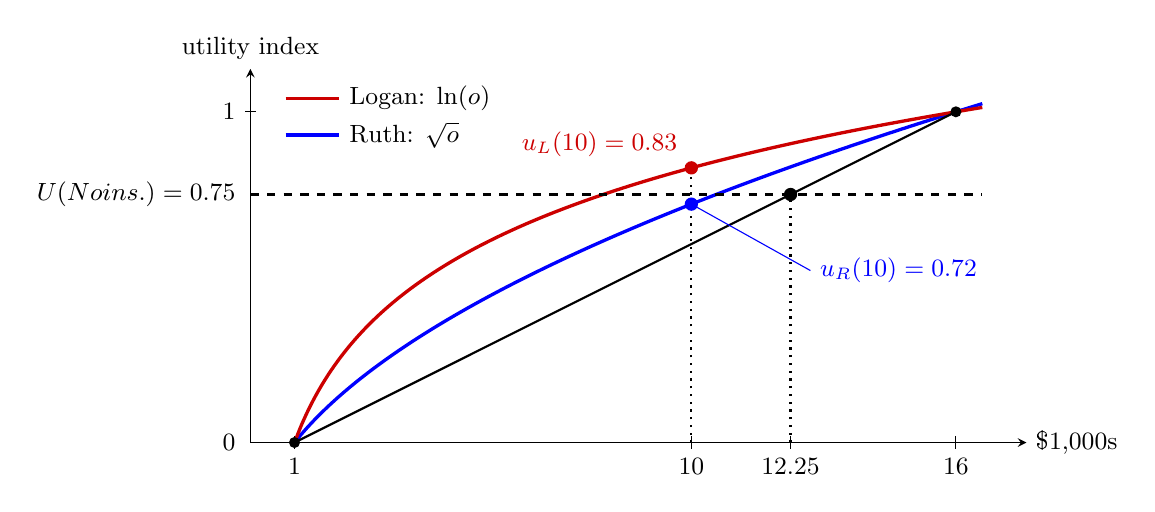
\begin{tikzpicture}[x=0.56cm, y=4.2cm, >=stealth]
  \draw[->] (0,0) -- (17.6,0) node[right] {\small \$1,000s};
  \draw[->] (0,0) -- (0,1.13) node[above] {\small utility index};
  \foreach \d in {1,16}{ \draw (\d,0.02) -- (\d,-0.02) node[below] {\small \d}; }
  \draw (0.12,1) -- (-0.12,1) node[left] {\small 1};
  \node[left] at (-0.12,0) {\small 0};
  \draw[blue, very thick, smooth, samples=100, domain=1:16.6] plot (\x,{(sqrt(\x)-1)/3});
  \draw[red!80!black, very thick, smooth, samples=100, domain=1:16.6] plot (\x,{ln(\x)/2.7726});
  \draw[red!80!black, very thick] (0.8,1.04) -- (2.0,1.04) node[right, black] {\small Logan: $\ln(o)$};
  \draw[blue, very thick] (0.8,0.93) -- (2.0,0.93) node[right, black] {\small Ruth: $\sqrt{o}$};
  \fill (1,0) circle (2pt);
  \fill (16,1) circle (2pt);
  \onslide<2->{
    \draw[thick] (1,0) -- (16,1);
    \draw (12.25,0.02) -- (12.25,-0.02) node[below] {\small 12.25};
    \draw[dotted, thick] (12.25,0) -- (12.25,0.75);
    \draw[dashed, thick] (0,0.75) -- (16.6,0.75);
    \node[left] at (-0.12,0.75) {\small $U(\text{No ins.})=0.75$};
    \fill (12.25,0.75) circle (2.4pt);
  }
  \onslide<3->{
    \draw (10,0.02) -- (10,-0.02) node[below] {\small 10};
    \draw[dotted, thick] (10,0) -- (10,0.8305);
    \fill[blue] (10,0.7208) circle (2.4pt);
    \fill[red!80!black] (10,0.8305) circle (2.4pt);
    \node[blue, anchor=west] (ur) at (12.7,0.52) {\small $u_R(10)=0.72$};
    \draw[blue, thin] (ur.west) -- (10,0.7208);
    \node[red!80!black, anchor=south east] at (9.9,0.835) {\small $u_L(10)=0.83$};
  }
\end{tikzpicture}
\bsk
\raggedright
\only<1>{Both rescaled so that $u(1)=0$ and $u(16)=1$. (Linear rescaling: allowed!)\\
Logan's curve bends more: Logan is \textbf{more} risk averse than Ruth.}%
\only<2>{No insurance: 75\% chance of the best, 25\% chance of the worst.\\
So $U(\text{No ins.})=0.75$ for \textbf{both} of them: the dashed line.}%
\only<3>{Insurance gives 10 for sure. Is $u(10)$ above or below the dashed line?\\
\textbf{Ruth:} below, so no insurance. \quad \textbf{Logan:} above, so buy insurance.}
\vfill
{\footnotesize Normalized: \ Ruth \ $u_R(o)=\tfrac13\sqrt{o}-\tfrac13$ \qquad Logan \ $u_L(o)=\tfrac{1}{\ln(16)}\ln(o)\approx 0.36\ln(o)$}
\vspace{-0.2in}
\end{frame}

\begin{frame}{How Much Would They Pay?}
The expected loss is \ $\tfrac14\times\$15{,}000=\$3{,}750$. \ Nationwide charges \$6,000.
\bsk
What's the \textbf{most} each would pay for full insurance?
\bsk
\begin{itemize}
    \item \textbf{Ruth:} find the sure wealth $w$ with $\sqrt{w}=3.25$
      \vspace{0.5in}
    \item \textbf{Logan:} find the sure wealth $w$ with $\ln(w)=\tfrac34\ln(16)$
      \vspace{0.5in}
\end{itemize}
{\footnotesize On the graph: where the dashed line crosses each curve.}
\vfill
\textbf{Lesson:} Knowing someone is risk averse doesn't tell you what they'll choose.\\
You need to know their utility index.
\vspace{-0.3in}
\end{frame}

% ==============================================================
% WORKED EXAMPLE
% ==============================================================
% Normalized index: u(M)=1, u(J)=0.5, u(D)=0.2, u(N)=0.
%   U(W1) = .5(.5)+.5(.2)          = 0.35
%   U(W2) = .3(1)+.7(0)            = 0.30
%   U(W3) = .1(1)+.4(.5)+.5(.2)    = 0.40      => W3 > W1 > W2
% v = 10u+5: (15, 10, 7, 5) -> 8.5, 8.0, 9.0   => same ranking
% w = u^2:   (1, .25, .04, 0) -> .145, .30, .22 => W2 > W3 > W1 (changed)
% Q5: can't say. Outcomes aren't numbers, so there is no expected value.
% ---------------------------------------------------------------------

\begin{frame}[standout]
Let's Work One Out
\end{frame}

\begin{frame}{The Prize Wheel}
Carmen gets one spin of a prize wheel at the Ohio Union. The possible prizes:
\begin{itemize}
    \item $M$: a ticket to the Michigan game \hspace{0.4in} $J$: a pint of Jeni's ice cream
    \item $D$: a dozen Buckeye Donuts \hspace{0.72in} $N$: nothing
\end{itemize}
Carmen's ranking: \ $M\succ J\succ D\succ N$. \ Carmen also tells us:
\begin{itemize}
    \item $J$ for sure is just as good as a 50\% chance of $M$ (otherwise $N$)
    \item $D$ for sure is just as good as a 20\% chance of $M$ (otherwise $N$)
\end{itemize}
\bsk
Carmen can pick which wheel to spin:
$$W_1=\begin{pmatrix} J & D \\[2pt] 0.5 & 0.5\end{pmatrix}
\qquad
W_2=\begin{pmatrix} M & N \\[2pt] 0.3 & 0.7\end{pmatrix}
\qquad
W_3=\begin{pmatrix} M & J & D \\[2pt] 0.1 & 0.4 & 0.5\end{pmatrix}$$
\vspace{-0.2in}
\end{frame}

\begin{frame}{The Prize Wheel}
\begin{enumerate}
    \item Write down Carmen's normalized utility index. \vspace{0.3in}
    \item Find the expected utility of each wheel. Which does Carmen spin? \vspace{0.45in}
    \item Rescale using $v(o)=10u(o)+5$. Does the ranking of wheels change? \vspace{0.35in}
    \item Now rescale using $w(o)=u(o)^2$. Does the ranking change? Why? \vspace{0.35in}
    \item Is Carmen risk averse, risk neutral, or risk loving? \vspace{0.2in}
\end{enumerate}
\end{frame}

\begin{frame}{What Have We Learned, Charlie Brown?}
\begin{itemize}
    \item \textbf{Expected value} needs numeric outcomes. \textbf{Expected utility} doesn't
    \item $u(o)$: \textbf{utility index} over outcomes
    \item $U(L)$: \textbf{expected utility} over lotteries
    \begin{itemize}
        \item $U(L)=p_1u(o_1)+\cdots+p_nu(o_n)$
    \end{itemize}
    \item The utility index can only be rescaled \textbf{linearly}
    \begin{itemize}
        \item So we can normalize: best outcome $=1$, worst outcome $=0$
    \end{itemize}
    \item Risk averse / neutral / loving $\iff$ $u(o)$ is concave / linear / convex
    \begin{itemize}
        \item Only for numeric outcomes!
    \end{itemize}
    \item Two risk-averse people can still make different choices
\end{itemize}
\vfill
Next: games where the payoffs are expected utilities
\vspace{-0.4in}
\end{frame}

\begin{frame}{Reading \& Practice}
\begin{itemize}
    \item Bonanno, \textit{Game Theory}, Chapter 5
    \begin{itemize}
        \item \S5.1 (risk attitudes) and \S5.2 (expected utility)
        \item \S5.3 (the axioms): optional, read it for fun
    \end{itemize}
    \item Remember: Bonanno's $U(o)$ is our $u(o)$. His $E[U(L)]$ is our $U(L)$
    \item Exercises: \S5.4.1 (risk attitudes) and \S5.4.2 (expected utility)
    \begin{itemize}
        \item Exercises 5.2 and 5.4: outcomes that aren't numbers
        \item Exercise 5.11: two risk-averse people who choose differently
    \end{itemize}
    \item Solutions in \S5.5
\end{itemize}
\vfill
\end{frame}

\end{document}
